\section{手順}
\subsection{課題1}
\subsubsection{計測対象}
\begin{itemize}
  \item 計測対象の選び方については、課題1だけを考えると任意のプログラムでよい。
  しかし、課題2でも課題1の計測結果が転用できることを考慮すると、処理結果が変わらないように、アルゴリズム
  だけを変更できるプログラムを選びたい。
  \begin{itemize}
    \item[→] 画像のノイズを除去することができる「
    3×3メディアンフィルタを使った平滑化」では、中央値を見つけるためにソートを行う。
    ソートに用いられるアルゴリズムは多数発見されているため、
    アルゴリズムを変更しやすい上に処理結果には影響しない。
    \begin{itemize}
      \item[→] 以上のことから、計測対象には、「
      3×3メディアンフィルタを使った平滑化」を選ぶことにする。
      具体的には、図\ref{graph:1}のようなプログラムを使う。
    \end{itemize}
  \end{itemize}
\end{itemize}
\begin{itemize}
  \item 画像処理に用いる画像の選び方については、任意の画像でよい。
  しかし、計測時間があまりにも長くならないようにするため、大きな画像は選ばない。
  また、画像の大きさや画素値などが計測時間にも影響すると考えられるため、
  全ての計測で使う画像は、1枚の同じ画像に統一して行う。
  \begin{itemize}
    \item[→] 今回の実験で使う画像は、大きさが「幅512ピクセル × 高さ479ピクセル」の
    図\ref{graph:2}のような画像「d850429avhrr4.bmp」である。
  \end{itemize}
\end{itemize}

\begin{figure}[hbtp]
  \begin{minipage}[t]{0.7\hsize}   
    \centering
    \caption{メディアンフィルタを使った平滑化のプログラム}
    \label{graph:1}
    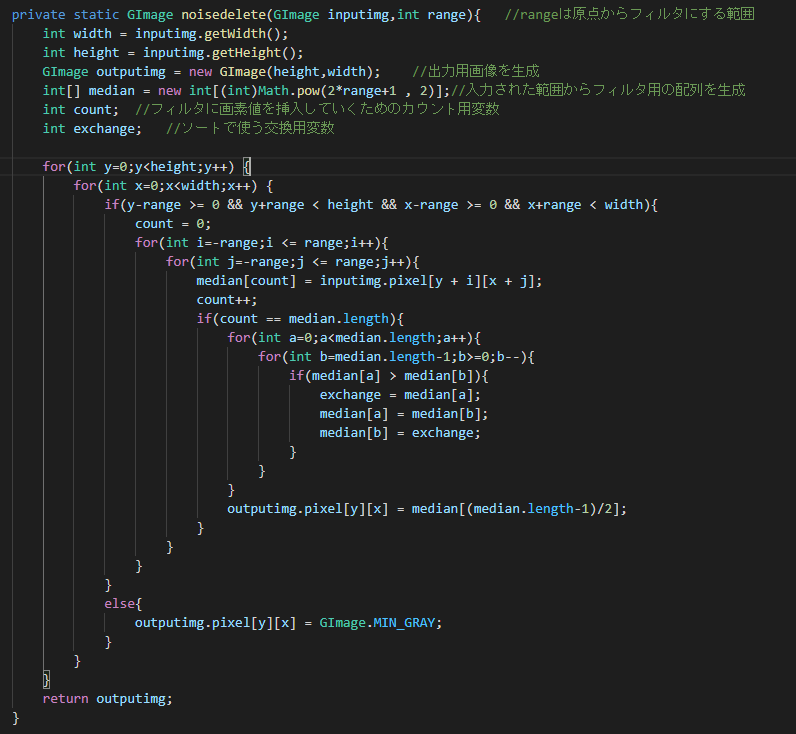
\includegraphics[scale = 0.6]{noisedeleteの中身1.PNG}
  \end{minipage}
  \begin{minipage}[t]{0.28\hsize}
    \centering
    \caption{計測対象の画像処理に使う画像}
    \label{graph:2}
    \includegraphics[scale = 0.3]{d850429avhrr4.bmp}
  \end{minipage}
\end{figure}

\clearpage

\subsubsection{計測方法}

\begin{enumerate}
  \item 計測方法の選択については、コストや精度の面から考えて、人力よりも
  コンピューター自体にやらせた方が効率がいいと判断したため、プログラミングで計測システムを作成する。
  \begin{itemize}
    \item[→] javaでは、「System.currentTimeMillis()」というメソッドを使うことで、long型で
  エポック秒(1970年1月1日0時0分0秒)から経過した時間をミリ秒単位で知ることができる。
  この実験では、このメソッドを利用して画像処理の処理時間を計測していく。
  \begin{itemize}
    \item[→] 具体的な計測方法は「計測したい処理」を
  「System.currentTimeMillis()」で囲いこむことで、処理前の時間と処理後の時間を取得する。
  そして、(2.1.1)の式のように処理後の時間から処理前の時間を引くことで、処理時間を計算する。
  \begin{equation}
    処理時間 = 処理後の時間 - 処理前の時間
  \end{equation}
  \end{itemize}
  \end{itemize}
  \item 次に、選択した計測方法が正確であるかどうかを判断できる条件を考える。
  \begin{itemize}
    \setlength{\leftskip}{1.0cm}
    \item[条件一] 今回の実験では、画像処理の処理時間だけを計測したいため、それ以外の処理の計測
    時間は排除したい。私が選択した計測方法で、画像処理の処理時間以外に、計測時間に反映され
    ると思われる処理は、計測に使うメソッドである「System.currentTimeMillis()」という処理自体
    が挙げられる。そのため、このメソッドに処理時間が存在するのかどうかを調べる。
    \item[条件二] 本題では、正解の処理時間が不明であるため、正確に処理時間が計測できて
    いるかどうかを判断することができない。そのため、処理時間が
    あらかじめ決められている処理を利用して、条件一の結果を含めた処理時間を正確に測れるか
    どうかをテストする。
    \item[条件三] 条件一、条件二は、私のコンピューターでの時間の進み方に依存しており
    、それが現実の時間の進み方と同じであるという前提で成り立っている。
    そのため、私のコンピューター以外の方法でも測ることで、前提が正しいかを調べた上で、
    プログラムに対して私の解釈違いが起こっていないかどうかも調べることができる。
  \end{itemize}
  
  \item 2で考えた条件を実際に確かめてみる。
  \begin{itemize}
    \item 条件一
    \begin{itemize}
      \item[方法] 計測方法は、図\ref{graph:3}のように、「System.currentTimeMillis()」を
      long型の変数「starttime」と「endtime」に入れる。
      その後、「endtime」から「starttime」を引いて
      処理時間を計算する。また、信頼性のあるデータをとるために、これらの処理をfor文で
      20回繰り返している。
      
      \item[結果] 「System.currentTimeMillis()」の処理時間の計測結果は、図\ref{graph:4}の
      ように、試行回数20回の全てで「0ms」となった。これらの結果より、
      「System.currentTimeMillis()」の処理時間はこの実験では考慮しなくてもよいと判断した。
      \begin{figure}[htbp]
        \begin{minipage}[t]{0.5\hsize}
          \centering
          \caption{「System.currentTimeMillis()」の処理時間を計測するプログラム}
          \label{graph:3}
          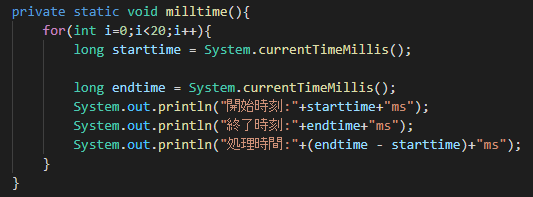
\includegraphics[scale=0.75]{milltimeのプログラム.PNG}
        \end{minipage}
        \begin{minipage}[t]{0.45\hsize}
          \centering
          \caption{「System.currentTimeMillis()」の処理時間の計測結果}
          \label{graph:4}
          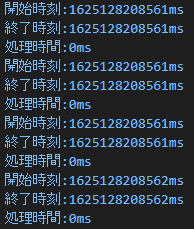
\includegraphics[scale=0.9]{milltimeの結果.PNG}
        \end{minipage}
      \end{figure}
    \end{itemize}
    \clearpage
    \item 条件二
    \begin{itemize}
      \item[方法] javaの「Thread.sleep();」メソッドでは、引数に入れた数字×ミリ秒だけ、プログラムを
      一時停止することができる。これを利用して「Thread.sleep();」を処理とみなして、処理時間を
      計測し、「Thread.sleep();」の引数との比較を行うことで、計測方法が正確かどうかを判断する。
      この実験では、「Thread.sleep();」の引数を「1000」として、
      計測処理をfor文で20回繰り返えす図\ref{graph:5}のような
      プログラムを作成して計測した。
      
      \item[結果] 結果は、図\ref{graph:6}のようになり、結果をまとめると
      「1001ms」が9回、他は全て「1000ms」となった。1msの誤差が約1/2の確率で発生したものの
      、この程度の誤差はマシンの性能などによる誤差の範疇だと考察できるため、
      この計測方法は正確であると判断した。
      \begin{figure}[htbp]
        \begin{minipage}[t]{0.5\hsize}
          \centering
          \caption{「Thread.sleep();」を用いた計測方法の正確さ確認のプログラム}
          \label{graph:5}
          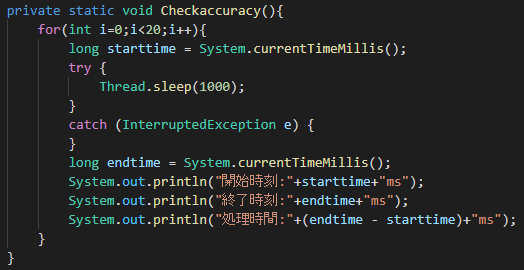
\includegraphics[scale=0.75]{計測方法の正確さを確認.PNG}
        \end{minipage}
        \begin{minipage}[t]{0.45\hsize}
          \centering
          \caption{「Thread.sleep();」を用いた計測方法の正確さ確認の出力結果}
          \label{graph:6}
          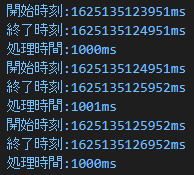
\includegraphics[scale=0.9]{計測方法の正確さを確認の出力.PNG}
        \end{minipage}
      \end{figure}
    \end{itemize}
    \item 条件三
    \begin{itemize}
      \item[方法] 
      計測に用いるコンピューターの機能で計測しても意味がないため、スマートフォンのストップウォッチを
      用いて手動で測る。手動のため「Thread.sleep();」の引数を長めの「20000」に設定し、
      開始と終了のログがでるように、図\ref{graph:7}のようなプログラムを使う。
      \item[結果] 
      ストップウォッチは、図\ref{graph:8}のように約20秒となった。「Thread.sleep();」の引数
      は「20000」であるため、「20000ミリ秒」を秒に換算すると「20秒」となる。
      つまり、ストップウォッチで測った時間と合致しているため、計測で使う
      コンピューターの時間の進み方は正しいと判断できる。また、コンピューターの計測結果でも
      「20000ms」となっていたことから、「Thread.sleep();」や
      「System.currentTimeMillis()」への解釈違いも起こっていないと判断することができた。
      \begin{figure}[htbp]
        \begin{minipage}[t]{0.5\hsize}
          \centering
          \caption{ストップウォッチを用いた計測方法の正確さ確認のプログラム}
          \label{graph:7}
          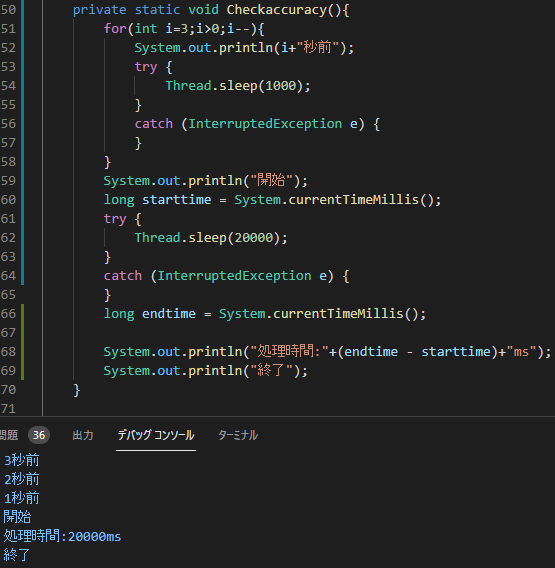
\includegraphics[scale=0.4]{計測方法の正確さを確認2.PNG}
        \end{minipage}
        \begin{minipage}[t]{0.45\hsize}
          \centering
          \caption{ストップウォッチを用いた計測方法の正確さ確認の結果}
          \label{graph:8}
          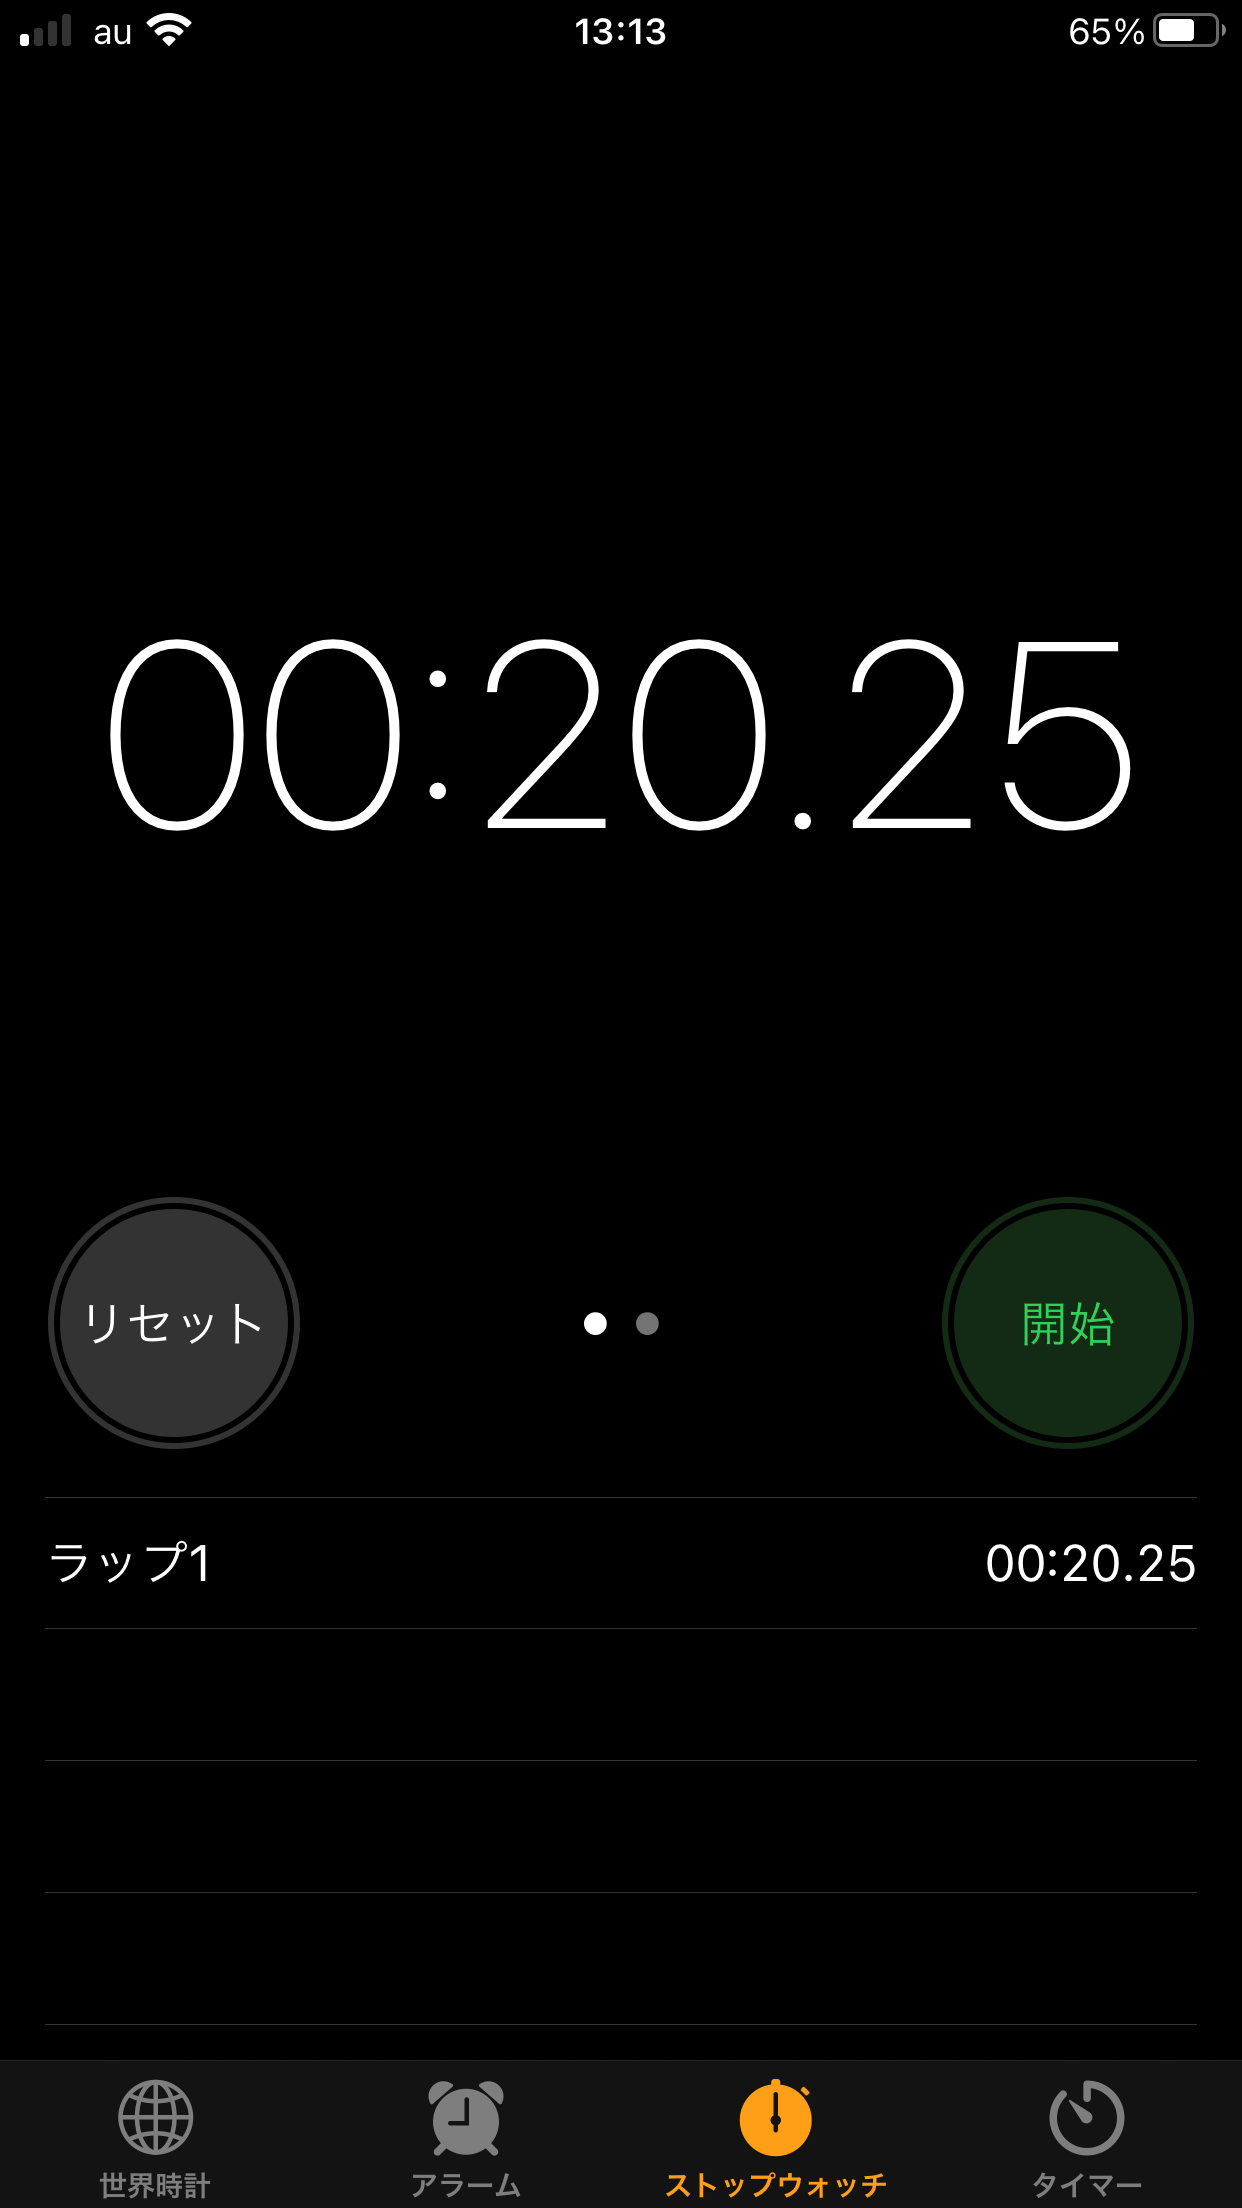
\includegraphics[scale=0.1]{計測方法の正確さを確認2結果.PNG}
        \end{minipage}
      \end{figure}
    \end{itemize}
  \end{itemize}
\item 3で、計測方法は正確であると判断できたため、本題の「
3×3メディアンフィルタを使った平滑化」を計測する。
\begin{itemize}
  \item[方法] テストプログラムから処理部分を「3×3メディアンフィルタを使った平滑化
  」のメソッドである「noisedelete()」に変更する。
  「noisedelete()」の引数は、図\ref{graph:9}のように
  「inputimg」には定義していた「d850429avhrr4.bmp」を入れて、「
  range」には、3×3フィルターを使うため「1」を入れる。
  \begin{figure}[htbp]
    \begin{minipage}[t]{\hsize}
      \centering
      \caption{「3×3メディアンフィルタを使った平滑化」の計測プログラム}
      \label{graph:9}
      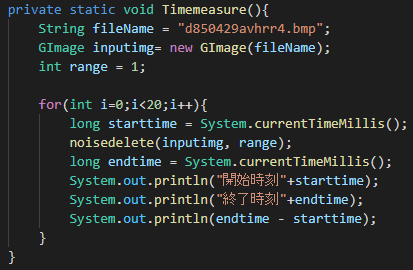
\includegraphics[scale=1]{課題1の計測1.PNG}
    \end{minipage}
  \end{figure}

\end{itemize}
  
\end{enumerate}
\clearpage

\subsection{課題2}
\subsubsection{計測対象}
\begin{itemize}
  \item 課題1と同様に、「3×3メディアンフィルタを使った平滑化」を使う。変更するアルゴリズム
  は、課題1で説明した通りにソート部分を変更する。図\ref{graph:10}は、課題1で使った
  プログラムのソートの部分を抜粋したものである。
  \begin{figure}[htbp]
    \begin{minipage}[t]{\hsize}
      \centering
      \caption{課題1プログラムのソート部分}
      \label{graph:10}
      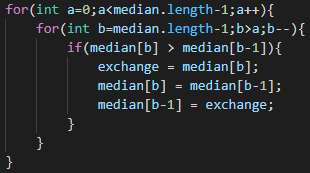
\includegraphics[scale=1]{課題2バブルソート.PNG}
    \end{minipage}
  \end{figure}

\end{itemize}

\subsubsection{計測方法}